\documentclass[czech,12pt,a4paper,titlepage]{article}
\usepackage[left=15mm,right=15mm,top=25mm,bottom=25mm]{geometry}
\usepackage[autostyle]{csquotes}
\usepackage[export]{adjustbox}
\usepackage[czech]{babel}
\usepackage{graphicx}
\usepackage{utopia}

\title{%
    \textbf {MelodySphere} \\
    \bigskip
    \large Projekt do předmětu Databázové systémy I}
\author{Kateřina Baierová}
\date{}

\begin{document}

    \graphicspath{ {./img/} }

    \begin{titlepage}
        \maketitle
        \thispagestyle{empty}
    \end{titlepage}

    \tableofcontents

    \clearpage


    \section{Specifikace zadání}\label{sec:specifikace-zadani}
    \subsection*{Vize}
    Cílem webové aplikace je poskytovat uživatelům prostředí pro přehrávání hudby.
    Uživatel si vytvoří svůj osobní účet, který mu umožní nejen poslouchat
    hudbu svých oblíbených umělců, ale také vytvářet
    vlastní playlisty nebo hodnotit jednotlivé skladby.

    Dále poskytujeme možnost registrovat se jako umělec,
    což uživatelům umožňuje aktivně přispívat do hudební komunity.
    Umělci mohou přidávat vlastní skladby a vytvářet hudební alba.

    Aplikace má také uživatelům usnadňovat vyhledávání různých hudebních žánrů
    a poskytovat informace o jednotlivých umělcích.


    \subsection*{Role}
    \textbf{Uživatel} je osoba, která vytváří a spravuje svůj osobní účet.
    Po registraci získává možnost poslouchat hudbu, vytvářet vlastní playlisty
    a hodnotit jednotlivé skladby.
    Uživatelé mohou využívat funkce jako vyhledávání hudebních žánrů nebo
    získávat informace o umělcích.


    \textbf{Umělec} je uživatel s registrovaným účtem, který má zájem aktivně přispívat do hudební komunity.
    Může přidávat vlastní skladby a vytvářet hudební alba, která jsou dostupná pro poslech ostatním uživatelům.
    Umělci mají možnost prezentovat svou tvorbu a budovat svůj profil.

    \subsection*{Vstupy}
    \textbf{Uživatelé} jsou klíčovou entitou v projektu.
    Registrací získávají možnost poslouchat hudbu, tvořit vlastní playlisty a hodnotit jednotlivé skladby.
    Jejich profily obsahují informace jako jméno, příjmení, kontaktní e-mail, zabezpečené heslo, premium status a datum registrace.


    Další důležitou entitou jsou \textbf{Umělci}, kteří mají svůj profil na platformě.
    Každý umělec má jméno, hudební žánr, místo původu a krátkou biografii.
    Jsou zodpovědní za přidávání nových skladeb a vytváření alb, která jsou dostupná pro poslech ostatním uživatelům.


    Entita \textbf{Skladba} obsahuje detaily o jednotlivých písních.
    Každá skladba má svůj název, délku, datum vydání, text (pokud existuje) a spojení s umělci, kteří na ní pracovali.
    Skladby mohou patřit do různých žánrů a být součástí alb.
    Uživatelé mohou hodnotit skladby, což se také eviduje jako součást této entity.


    Dvě další entity jsou \textbf{Playlisty} a \textbf{Alba}.
    Playlisty jsou vytvářeny uživateli a mohou obsahovat různé skladby z různých alb a umělců.
    Alba jsou kolekcemi skladeb vytvořenými umělci, která jsou k dispozici pro poslech ostatním uživatelům.
    Každé album může obsahovat skladby od jednoho nebo více umělců.


    Kromě toho, existují entity jako \textbf{Hodnocení} a \textbf{Žánry}.
    Hodnocení zaznamenává hodnocení skladby uživateli, což umožňuje vyhodnocení oblíbenosti skladeb.
    Žánry určují hudební žánry spojené s umělci a jednotlivými skladbami, což pomáhá organizovat hudbu a usnadňuje uživatelům vyhledávání specifických žánrů.

    \clearpage

    \subsection*{Výstupy}
    Pro umělce je k dispozici například výstup, který umožňuje zobrazit jeho skladby vytvořené v určitém období a setřídit je podle hodnocení.
    Umělec může specifikovat časové období, například poslední rok nebo konkrétní měsíc, a získat seznam svých skladeb v tomto období.
    Tyto skladby budou seřazeny podle hodnocení, kde nejlépe hodnocené skladby budou na vrcholu seznamu.
    To umožní umělci zhodnotit, jaké skladby z daného období měly největší ohlas u posluchačů.

    Uživatelé mají možnost vyhledávat nejnovější hudební alba na základě data jejich přidání a současně je filtrovat třeba podle svých oblíbených hudebních žánrů.
    Tato funkce jim umožňuje zadat specifické datum a zobrazit alba, která byla přidána od té doby, a to ještě více omezit na alba v žánrech.


    Pro administrátora je k dispozici třeba přehled statistik týkající se uživatelů a plateb za prémiové služby.
    Administrátor má možnost sledovat statistiky, jako je počet nově zaregistrovaných uživatelů v různých časových obdobích.
    Dále může získat informace o počtu uživatelů, kteří zakoupili prémiové členství, a sledovat trendy růstu nebo poklesu v registracích či nákupu prémiového členství.

    \subsection*{Funkce}
    Kolaborativní tvorba playlistů umožňuje uživatelům společně vytvářet a úpravovat playlisty s ostatními uživateli.
    Tato funkce podporuje sdílení playlistů a spolupráci na jejich obsahu a úpravách.
    Pro zajištění kvality obsahu playlistů a minimalizaci chyb systém provádí kontrolu unikátnosti skladeb.
    Při přidání nové skladby do playlistu ověřuje, zda již skladba v playlistu není obsažena, přičemž upozorní
    uživatele na možnost duplicity a umožní mu potvrzení nebo zrušení přidání.
    Taktéž systém monitoruje dostupnost skladeb v playlistu a v případě, že některá skladba není momentálně dostupná,
    nabídne uživateli možnost nahrazení jinou skládankou.
    Dále zabezpečuje integritu playlistů během společné editace, takže při práci více uživatelů
    zároveň se snaží zabránit duplicitním změnám a konfliktním situacím.
    Tímto způsobem systém uživatelům umožňuje vytvářet obsáhlé a rozmanité playlisty díky společné tvorbě a úpravám obsahu,
    zatímco zároveň minimalizuje možnost výskytu chyb a duplikací skladeb.
    \clearpage


    \section{Datová analýza}\label{sec:datova-analyza}
    \subsection*{Konceptuální datový model}
    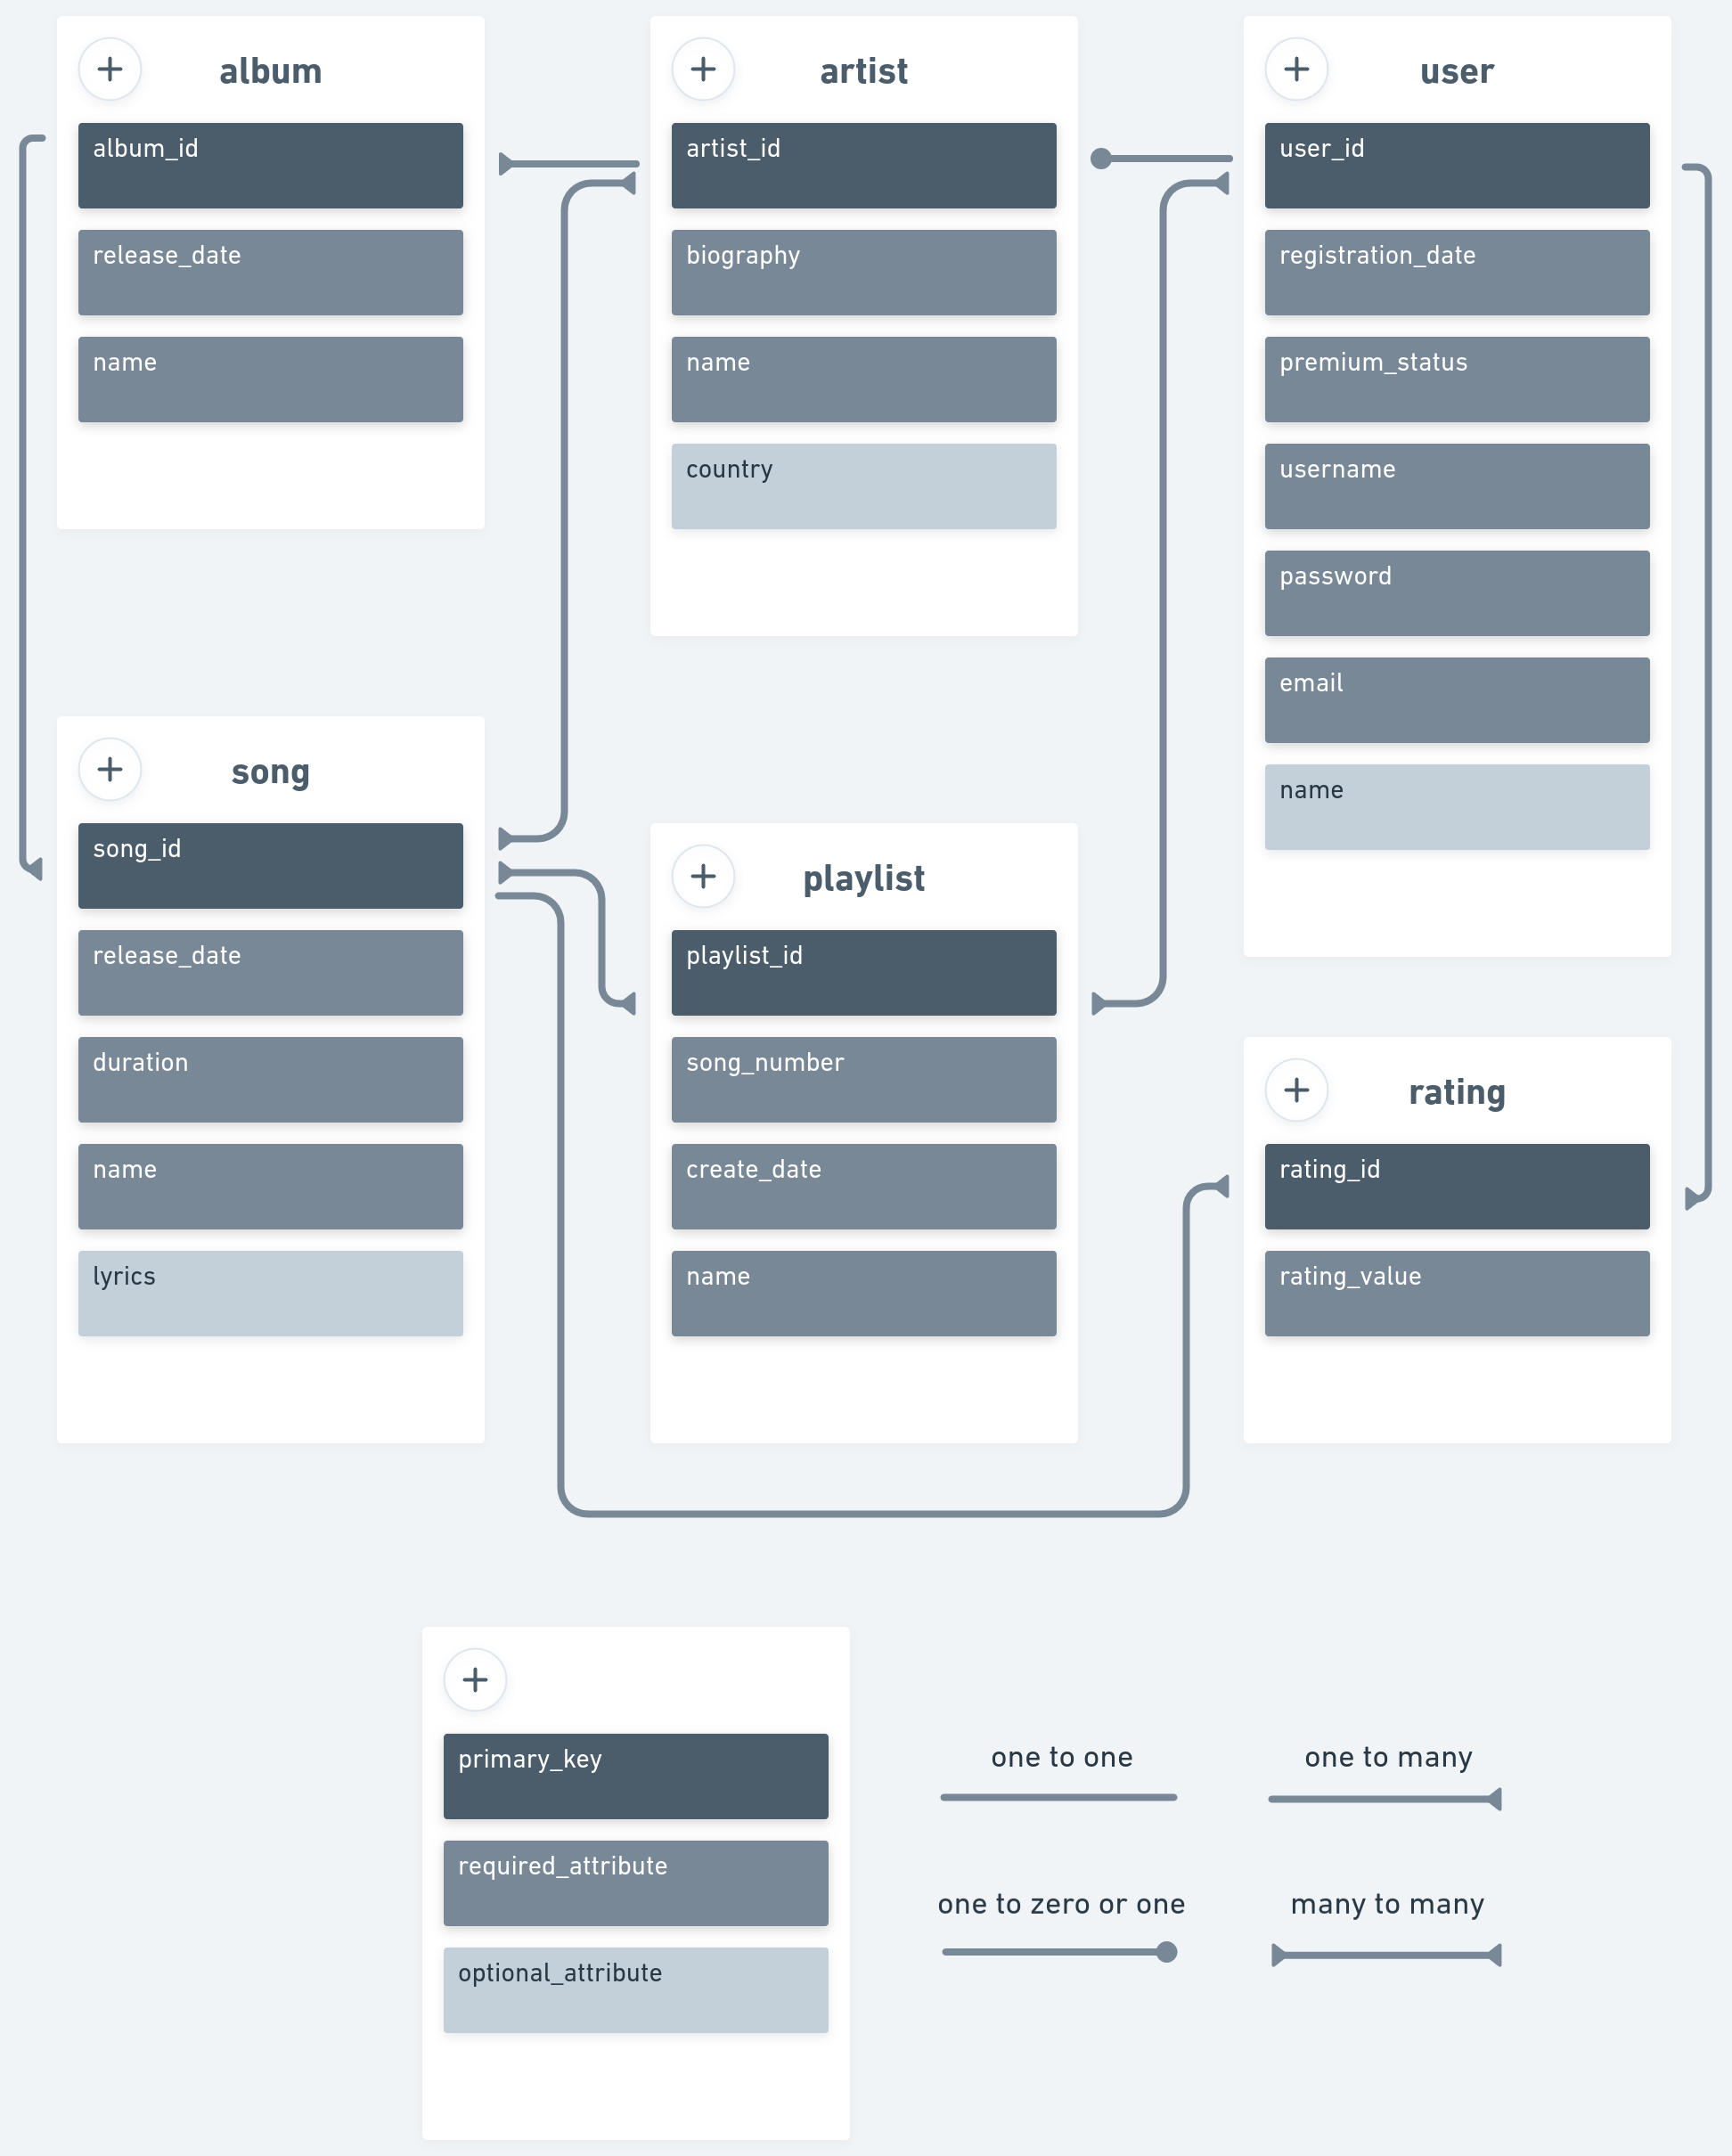
\includegraphics[width=0.9 \textwidth, center]{konceptualni_datovy_model}

    \subsection*{Relační datový model}
    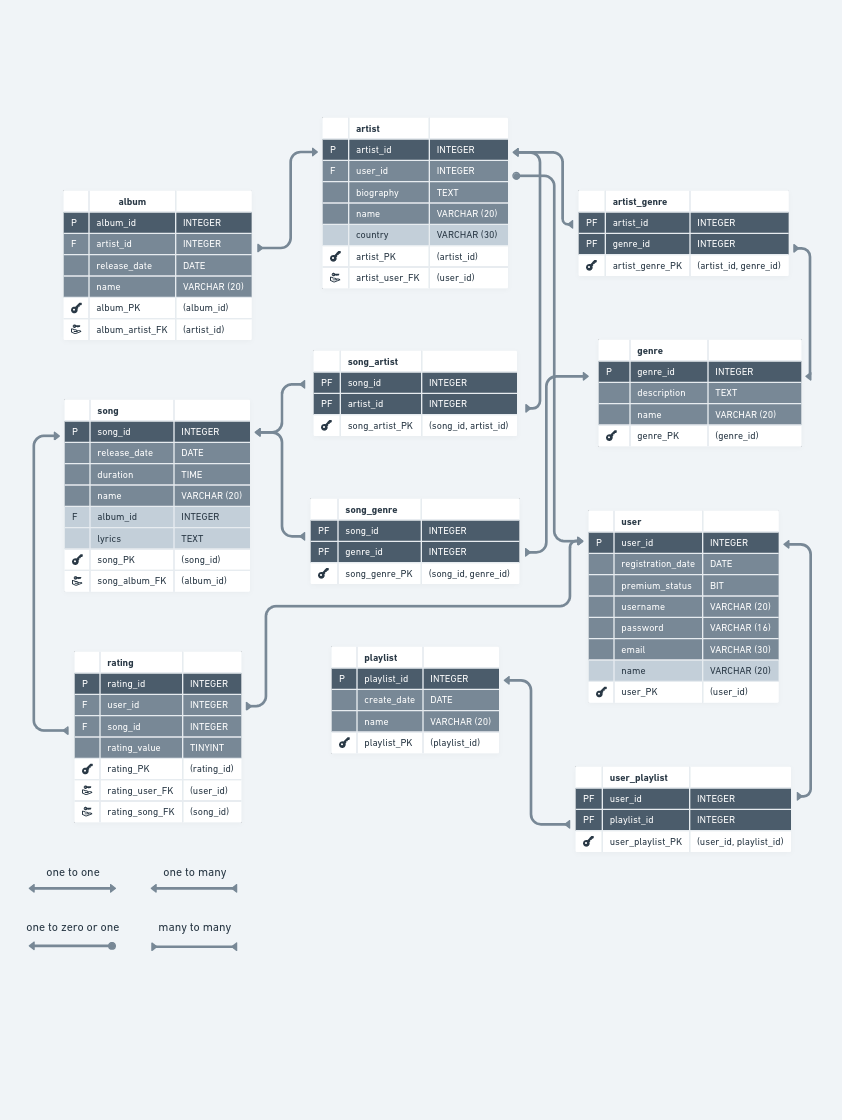
\includegraphics[width=1\textwidth, center]{relacni_datovy_model}

    \clearpage

    \section*{Datový slovník}
    Popis jednotlivých tabulek je uveden v následujícím datovém slovníku.

\subsection*{User}
\begin{tabular}{ |c|c c c c c|c| }
    \hline
    \textbf{Název atributu} & \textbf{Datový typ} & \textbf{Délka} & \textbf{Klíč} & \textbf{Null} & \textbf{IO} & \textbf{Popis}                         \\
    \hline
    user\_id                & INTEGER             &                & Primární      & Ne            &             & Automaticky inkrementovaný PK   \\
    registration\_date      & DATE                &                &               & Ne            &             & Datum registrace uživatele      \\
    premium\_status         & BIT                 &                &               & Ne            &             & Status prémiového účtu          \\
    username                & VARCHAR             & 20             &               & Ne            &             & Přezdívka uživatele             \\
    password                & VARCHAR             & 16             &               & Ne            & 3           & Heslo uživatele                 \\
    email                   & VARCHAR             & 30             &               & Ne            &             & E-mail uživatele pro přihlášení \\
    name                    & VARCHAR             & 20             &               & Ano           &             & Jméno uživatele                 \\
    \hline
\end{tabular}
\bigskip

\subsection*{Song}
\begin{tabular}{ |c|c c c c c|c| }
    \hline
    \textbf{Název atributu} & \textbf{Datový typ} & \textbf{Délka} & \textbf{Klíč} & \textbf{Null} & \textbf{IO} & \textbf{Popis}                         \\
    \hline
    song\_id                & INTEGER             &                & Primární      & Ne            &             & Automaticky inkrementovaný PK   \\
    release\_date           & DATE                &                &               & Ne            &             & Datum vydání skladby            \\
    duration                & TIME                &                &               & Ne            & 1           & Délka skladby                   \\
    name                    & VARCHAR             & 20             &               & Ne            &             & Název skladby                   \\
    album\_id               & INTEGER             &                & Cizí (Album)  & Ano           &             & Album, do kterého skladba patří \\
    lyrics                  & TEXT                &                &               & Ano           &             & Text ke skladbě                 \\
    \hline
\end{tabular}
\bigskip

\subsection*{Artist}
\begin{tabular}{ |c|c c c c c|c| }
    \hline
    \textbf{Název atributu} & \textbf{Datový typ} & \textbf{Délka} & \textbf{Klíč} & \textbf{Null} & \textbf{IO} & \textbf{Popis}                         \\
    \hline
    artist\_id              & INTEGER             &                & Primární      & Ne            &             & Automaticky inkrementovaný PK \\
    user\_id                & INTEGER             &                & Cizí (User)   & Ne            &             & Správce účtu                  \\
    biography               & TEXT                &                &               & Ne            &             & Biografie tvůrce              \\
    name                    & VARCHAR             & 20             &               & Ne            &             & Jméno tvůrce                  \\
    country                 & VARCHAR             & 30             &               & Ano           &             & Země původu                   \\
    \hline
\end{tabular}
\bigskip

\subsection*{Album}
\begin{tabular}{ |c|c c c c c|c| }
    \hline
    \textbf{Název atributu} & \textbf{Datový typ} & \textbf{Délka} & \textbf{Klíč} & \textbf{Null} & \textbf{IO} & \textbf{Popis}                         \\
    \hline
    album\_id               & INTEGER             &                & Primární      & Ne            &             & Automaticky inkrementovaný PK \\
    artist\_id              & INTEGER             &                & Cizí (Artist) & Ne            &             & Tvůrce alba                   \\
    release\_date           & DATE                &                &               & Ne            &             & Datum vydání alba             \\
    name                    & VARCHAR             & 20             &               & Ne            &             & Jméno alba                    \\
    \hline
\end{tabular}
\bigskip

\subsection*{Rating}
\begin{tabular}{ |c|c c c c c|c| }
    \hline
    \textbf{Název atributu} & \textbf{Datový typ} & \textbf{Délka} & \textbf{Klíč} & \textbf{Null} & \textbf{IO} & \textbf{Popis}                         \\
    \hline
    rating\_id              & INTEGER             &                & Primární      & Ne            &             & Automaticky inkrementovaný PK \\
    user\_id                & INTEGER             &                & Cizí (User)   & Ne            &             & Hodnotící uživatel            \\
    song\_id                & INTEGER             &                & Cizí (Song)   & Ne            &             & Hodnocená skladba             \\
    rating\_value           & TINYINT             &                &               & Ne            & 2           & Samotné ohodnocení            \\
    \hline
\end{tabular}
\bigskip

\subsection*{Playlist}
\begin{tabular}{ |c|c c c c c|c| }
    \hline
    \textbf{Název atributu} & \textbf{Datový typ} & \textbf{Délka} & \textbf{Klíč} & \textbf{Null} & \textbf{IO} & \textbf{Popis}                         \\
    \hline
    playlist\_id            & INTEGER             &                & Primární      & Ne            &             & Automaticky inkrementovaný PK \\
    create\_date            & DATE                &                &               & Ne            &             & Datum vytvoření playlistu     \\
    name                    & VARCHAR             & 20             &               & Ne            &             & Název playlistu               \\
    \hline
\end{tabular}
\bigskip

\subsection*{Song\_artist}
\begin{tabular}{ |c|c c c c c|c| }
    \hline
    \textbf{Název atributu} & \textbf{Datový typ} & \textbf{Délka} & \textbf{Klíč} & \textbf{Null} & \textbf{IO} & \textbf{Popis}                         \\
    \hline
    song\_id                & INTEGER             &                & Cizí (Song)   & Ne            &             & Vytvořená skladba \\
    artist\_id              & INTEGER             &                & Cizí (Artist) & Ne            &             & Tvůrce skladby    \\
    \hline
\end{tabular}
\bigskip

\subsection*{Song\_playlist}
\begin{tabular}{ |c|c c c c c|c| }
    \hline
    \textbf{Název atributu} & \textbf{Datový typ} & \textbf{Délka} & \textbf{Klíč}   & \textbf{Null} & \textbf{IO} & \textbf{Popis}                         \\
    \hline
    song\_id                & INTEGER             &                & Cizí (Song)     & Ne            &             & Daná skladba   \\
    playlist\_id            & INTEGER             &                & Cizí (Playlist) & Ne            &             & Dany laylist   \\
    \hline
\end{tabular}
\bigskip

\subsection*{User\_playlist}
\begin{tabular}{ |c|c c c c c|c| }
    \hline
    \textbf{Název atributu} & \textbf{Datový typ} & \textbf{Délka} & \textbf{Klíč}   & \textbf{Null} & \textbf{IO} & \textbf{Popis}                         \\
    \hline
    user\_id                & INTEGER             &                & Cizí (USer)     & Ne            &             & Tvůrce playlistu   \\
    playlist\_id            & INTEGER             &                & Cizí (Playlist) & Ne            &             & Vytvořený playlist \\
    \hline
\end{tabular}
\bigskip

\subsubsection*{Integritní omezení:}
\begin{enumerate}
    \item \textit{duration} musí mít maximálně 15 minut.
    \item \textit{rating\_value} může nabýt pouze hodnoty 1--5.
    \item \textit{password} musí obsahovat minimálně 6 znaků.
\end{enumerate}

\end{document}
